\chapter{Decision-Theoretic Planning}
\label{ch:background}
% Introduction on what is Decision-Theoretic Planning
Automated \acrfull{acr:sdm} comprises the central problem of planning under uncertainty. 
\acrfull{acr:dtp} is concerned with the design of plans or \textit{policies} for settings in which uncertainty exists about the effects of actions, where the decision maker or \textit{agent} has incomplete information about the environment and its initial conditions, and where trade-offs need to be made between potentially conflicting objectives to determine an optimal course of action.
% <To be determined>
% Chapter organized as follows: section x....

\section{General Problem Formulation}
\label{sec:problem-formulation}
% Formulation of what kind of planning problems are considered in Decision-Theoretic Planning

The class of problems that are considered in \acrlong{acr:dtp} are those that require optimal stochastic control through the actions of decision maker(s), referred to as \textit{agent(s)}, in systems whose dynamics can be modeled as \textit{stochastic processes} \cite{Boutilier1999}.
The agent(s) in these systems sequentially need to choose from a set of actions that influence the system's behavior, consequently making the system switch from one state to another.
In these settings the system's current state and the agent's choice of action determines the probability distribution over the states the system might reach next.
In addition, the agent(s) might be uncertain about the system's current state, implying the need to infer from observations and making decisions based on probabilistic estimates of the system's state.

Typically the problems under consideration involve certain objectives to be achieved (e.g., tasks to be fulfilled) or properties to be satisfied (e.g., avoiding certain system states). 
Therefore the agent should decide on a optimal plan or \textit{policy} which makes it most likely for the system to reach its targets, while minimizing the risk of producing undesirable states and the accompanied costs of the policy.
To find such a policy for \acrlong{acr:sdm} problems, a typical approach is to first setup a probabilistic model of the system and then apply a \acrshort{acr:dtp} algorithm on this model.
This probabilistic model comprises a system representation which defines the state space in terms of a set of multi-valued features, the set of actions for the agent to select together with the associated uncertainty defined by transition-probabilities, and a goal specification or performance metric regularly expressed by means of a reward structure.

Overall \acrshort{acr:dtp} aims to devise planning algorithms for planning under uncertainty, a problem that is addressed in numerous different fields of research such as AI planning and control theory.
In particular difficulties arise when planning techniques are applied to determine courses of action for real-world settings, such as % TODO

\section{System Representations: Markov Models}
\label{sec:system-representation}
% Definitions of Markov Models relevant as probabilistic models for planning under uncertainty

As the class of problems considered in \acrshort{acr:dtp} oft to present considerable structure, there exist various proposed solutions for planning under uncertainty that apply model-based approaches.
This type of decision-theoretic planner uses a stochastic model of the environment in which the agent operates, which compasses the uncertainty that is associated with the agent's actions, observations and the exogenous events that might occur.
Typically the uncertainty is modeled by establishing a \textit{state space} for the system accompanied by a set of possible \textit{transitions} between the states that might be induced with a certain probability by an agent executing \textit{actions}.
The most common types of stochastic models that are used in \acrshort{acr:dtp} are called \textit{Markov Models} (sometimes also referred to as \textit{Markovian Models}), which has been motivated by their success in other fields such as speech recognition \cite{baker1992large, gales2008application, rabiner1989tutorial} and reinforcement learning techniques \cite{Brafman2002}. %TODO Add more citations for RL
A Markov Model is a stochastic model in which the future states only depend on a limited number of prior observations. In fact, mostly processes or systems are modeled by Markov Models that satisfy the \textit{Markov Property}, which means that the state transitions are independent of any previous states or agent actions.

In the remainder of this section the most common types of discrete-state Markov Models are discussed one by one, starting from the fundamental models known as \textit{Markov Chains} in \autoref{subsec:markov-chains}, followed by their extension of \textit{\acrfullpl{acr:hmm}} in \autoref{subsec:hidden-markov-models}.
This again is followed by a discussion of the discrete-state Markov Models most relevant in \acrshort{acr:dtp}, being \textit{\acrfullpl{acr:mdp}} in \autoref{subsec:mdps} and their extension of \textit{\acrfullpl{acr:pomdp}} in \autoref{subsec:pomdps}.
%Finally in \autoref{subsec:other-markov-models} other related state space models are briefly discussed.

\subsection{Markov Chains}
\label{subsec:markov-chains}
% Markov Chains: States and Transitions

The evolution of system or processes can be viewed as so-called \textit{time-series}, in which a set of data-points can be ordered using an underlying physical dimension, typically time \cite{barberBRML2012}.
Formally, time-series can be defined as a series $x_{a:b}$ of data-points, with $x_{a:b} \equiv x_a, x_{a+1}, \ldots, x_b$.
By means of these time-series, probabilistic models can be devised for real-world systems or processes, by introducing the notion of \textit{states} as a description of the system at a particular point in time or \textit{stage}.

On the basis of the class of Markov Models lies the simplifying assumption that each state is only dependent on a limited number of previous states.
Under this assumption a \textit{Markov Chain} (or \textit{Markov Process}) can be defined as a model of a series $q_{1:T}$ of transitions between states $q_i$ drawn from a state space $\mathcal{S} = \{s_1,\ldots,s_n\}$. The initial state $q_1$ of a Markov Chain typically is either fixed or drawn from $\mathcal{S}$ using a probability distribution over initial states.
For the states or variables of a Markov Chain, the earlier mentioned assumption implies the following conditional independence to hold:
\begin{equation}
	p(q_t \vert q_1,\ldots,q_{t-1}) = p(q_t \vert q_{t - L}, \ldots, q_{t-1})
\end{equation}
where $L$ is the so-called \textit{order} of the Markov Chain.
% See summary barberBRML2012

\begin{figure}[ht!]
	\captionsetup[subfigure]{justification=centering}
	\centering
	\subcaptionbox{First-order Markov Chain.\label{fig:markov-chains-first-order}}{\begin{tikzpicture}[->,>=stealth',auto,node distance=2cm]
		\tikzstyle{every state}=[fill=white,draw=black,text=black,scale=1,double]	% thick
		\node[state] (s1) {$q_1$};
		\node[state] (s2) [right of=s1] {$q_2$};
		\node[state] (s3) [right of=s2] {$q_3$};
		\coordinate (con) at (0,2);
		\path
		(s1)
		edge node {} (s2)
		(s2)
		edge node {} (s3)
		(s3);
		\draw [->, dashed, shorten >=0pt] (s3) to[right] node[auto] {} ++(1.3,0)
		;
		\end{tikzpicture}} \quad
		\subcaptionbox{Second-order Markov Chain.\label{fig:markov-chains-second-order}}{\begin{tikzpicture}[->,>=stealth',auto,node distance=2cm]
		\tikzstyle{every state}=[fill=white,draw=black,text=black,scale=1,double]	% thick
		\node[state] (s1) {$q_1$};
		\node[state] (s2) [right of=s1] {$q_2$};
		\node[state] (s3) [right of=s2] {$q_3$};
		\node[state] (s4) [right of=s3] {$q_4$};
		\path
		(s1)
		edge node {} (s2)
		(s2)
		edge node {} (s3)
		(s1)
		edge [bend left] node {} (s3)
		(s3)
		edge node {} (s4)
		(s2)
		edge [bend left] node {} (s4)
		;
		\draw [->, dashed, shorten >=0pt] (s4) to[right] node[auto] {} ++(1.3,0)
		;
		\end{tikzpicture}}
	\caption{Graphical representation of different types of Markov Chains.}
	\label{fig:markov-chains}
\end{figure}

As depicted in \autoref{fig:markov-chains}, Markov Chains of different order can be defined. \autoref{fig:markov-chains-first-order} exemplifying a first-order Markov Chain, in which each state only depends on the previous state, and \autoref{fig:markov-chains-second-order} showing a second-order Markov Chain, in which each state depends on the two prior states of the Markov Chain.
In the special case where the transition distribution is independent of the stage of the system, but solely on the prior state(s), one speaks of a \textit{stationary} or \textit{homogeneous} Markov Chain.

Though, mostly first-order Markov Chains as depicted in \autoref{fig:markov-chains-first-order}, which are said to satisfy the \textit{Markov Property}, are applied widely for modeling stochastic processes, such as physical phenomena and economic time-series \cite{bacciu2015probabilistic}.
In addition, mostly compact, stationary, discrete-time, finite-space Markov Chains are used, bearing in mind the computational adequacy of the model (i.e., the larger the state space and order, the more computational cost might be incurred).
Some concrete examples of practical applications include assessing the reliability and/or safety of appliances in engineering \cite{cochran2001generic, cronvall2009combining,el2008optimal}, modeling water flows \cite{parent1991stochastic}, or modeling loan defaults \cite{grimshaw2011markov} in the financial world (for an overview see \cite{pasanisi2012estimating}).

In these chains the state transition probabilities can be stored in an $n \times n$ transition matrix $\mat{A} = [a_{ij}]$ with each entry
\begin{equation}
	a_{ij} = p(q_{t+1} = s_i\vert q_t = s_j)
\end{equation}
denoting the probability of state $s_i$ following state $s_j$.
Similarly, the initial state probabilities can be recorded in an $n \times 1$ initial state vector $\arr{\pi} = [\pi_i]$ with each entry
\begin{equation}
	\pi_i = p(q_1 = s_i)
\end{equation} 
denoting the probability of state $s_i$ being the initial state of the model.
Putting these components all together, a discrete stationary first-order Markov Chain can be defined as a 3-tuple $\mathcal{M} = (\mathcal{S}, \mat{A}, \arr{\pi})$ with $\mathcal{S}$ as state space, $\mat{A}$ as transition matrix and $\arr{\pi}$ as initial state vector.

\subsubsection*{Fitting Markov Chains}
There exist efficient methods for fitting a discrete stationary first-order Markov Chain provided a collected dataset describing the evolution of a stochastic process either by applying maximum likelihood (e.g., see \cite{bacciu2015probabilistic, barberBRML2012, lee1968maximum, teodorescu2009maximum}) or Bayesian inference (e.g., see \cite{barberBRML2012, lee1968maximum, minka2003bayesian}).
These methods estimate the transition distribution to fit a Markov Chain on a collected sequence of time-ordered states. 

The first-mentioned approach of likelihood maximization, works by estimating the transition probabilities by counting the observed transitions in the state sequence.
That is, if we let $n_{ij}$ denote the number of observed transitions from state $s_j$ to state $s_i$, then the maximum-likelihood estimation of the corresponding transition probability is
\begin{equation}
	p(q_{t+1} = s_i\vert q_t = s_j) = \frac{n_{ij}}{\sum_j n_{ij}}
\end{equation}

The second-mentioned approach of Bayesian inference is more suitable for many real-life problems, for which state sequences are incomplete, i.e. states are recorded only for certain stages, meaning there might be gaps in-between.
This type of approach aims to make an estimation of the transition probabilities by adopting a prior for the transition matrix $\mat{A}$, a convenient choice being a factorized prior from the product of $n$ independent \textit{Dirichlet} distributions, one for each row $\mat{A}_j$ such that:
\begin{equation}
	p(\mat{A}) = \prod_{j} \text{Dir}(\mat{A}_j \vert \alpha_j)
\end{equation}
parametrized by a vector $\arr{\alpha}$ with $\alpha_j > 0$ \cite{pasanisi2012estimating,barberBRML2012}.

\subsection{Hidden Markov Models}
\label{subsec:hidden-markov-models}
% Hidden Markov Models: Observations (partially observable) 
% also called latent
% inference problems
% shortly discuss the succesful applications see \cite{barberBRML2012} speech recognition, object tracking, genetic sequence analysis and add citations to the corresponding works

The Markov Chain model discussed in \autoref{subsec:markov-chains} requires the modeled system or stochastic process to be fully observable, meaning that each of its states correspond directly to an observation.
However, it is not unusual to encounter real-world systems in which the states are assumed to be unobservable, though are correlated with observable events produced by the system.
These systems can be modeled by a \acrfull{acr:hmm} in which the states, typically referred to as \textit{hidden} or \textit{latent} variables $h_{1:T}$, are unknown.
Additionally this model consists of observations, typically referred to as \textit{observed} or \textit{visible} variables $v_{1:T}$, which are dependent on the hidden variables through an emission $p(o_t\vert h_t)$ graphically depicted in \autoref{fig:hmm}. All by all a stationary \acrshort{acr:hmm}
consists of the following parts:

\begin{itemize}
	\item a discrete set of $n$ attainable states $\mathcal{S} = \{s_1, \ldots, s_n\}$, i.e. the underlying \textit{state space}
	\item a set of $m$ possible observations, $\mathcal{V} = \{v_1, \ldots, v_m\}$, i.e. the \textit{observation space}
	\item an $n \times n$ transition matrix $\mat{A} = [a_{ij}]$ defining the models' \textit{transition distribution} in which $a_{ij} = p(h_{t+1} = s_i \vert h_t = s_j)$ is the probability of state $s_i$ following state $s_j$ ($s_i, s_j \in \mathcal{S}$)
	\item an $m \times n$ emission matrix $\mat{B} = [b_{ij}]$ defining the models' \textit{emission distribution} in which $b_{ij} = p(o_t = v_i \vert h_t = s_j)$ the probability of observing $v_i$ from state $s_j$ ($v_i \in \mathcal{V}$, $s_j \in \mathcal{S}$)
	\item an $n \times 1$ initial state array $\arr{\pi} = [\pi_i]$ in which $\pi_i = p(h_1 = s_i)$ is the probability of having $s_i$ as the initial state ($s_i \in \mathcal{S}$)
\end{itemize}
Putting all of these components together, a stationary \acrshort{acr:hmm} can be defined as a 5-tuple $\mathcal{M} = (\mathcal{S}, \mathcal{V}, \arr{\pi}, \mat{A}, \mat{B})$ with $\mathcal{S}$ as state space, $\mathcal{V}$ as observation space, $\arr{\pi}$ as initial state vector, $\mat{A}$ as transition matrix and $\mat{B}$ as emission matrix.

\begin{figure}
	\centering
	\begin{tikzpicture}[->,>=stealth',auto,node distance=2cm]
	\tikzstyle{every state}=[fill=white,draw=black,text=black,scale=1,double]	% thick
	\node[state] (h1) {$h_1$};
	\node[state] (h2) [right of=h1] {$h_2$};
	\node[state] (h3) [right of=h2] {$h_3$};
	\node[state, draw=none] (dots) [right of=h3] {$\symbf{\cdots}$};
	\node[state] (ht) [right of=dots] {$h_t$};
	\node[state,fill={rgb:black,1;white,10}] (o1) [below of=h1] {$o_1$};
	\node[state,fill={rgb:black,1;white,10}] (o2) [below of=h2] {$o_2$};
	\node[state,fill={rgb:black,1;white,10}] (o3) [below of=h3] {$o_3$};
	\node[state,fill={rgb:black,1;white,10}] (ot) [below of=ht] {$o_t$};
	\path
	(h1)
	edge node {} (h2)
	(h2)
	edge node {} (h3)
	(h3)
	edge node {} (dots)
	(dots)
	edge node {} (ht)
	(h1)
	edge node {} (o1)
	(h2)
	edge node {} (o2)
	(h3)
	edge node {} (o3)
	(ht)
	edge node {} (ot)
	;
	\end{tikzpicture}
	\caption{Graphical representation of an \acrshort{acr:hmm} with hidden states $h_t \in \mathcal{S}$ and observations $o_t \in \mathcal{V}$ for $t = 1:T$}
	\label{fig:hmm}
\end{figure}

In practice \acrshortpl{acr:hmm} have a wide range of applications. One example is that of object tracking in which inference algorithms for \acrshortpl{acr:hmm} are used to estimate the (unknown) position of objects by a sequence of observations \cite{caelli2001shape}. Another well-known application example of \acrshortpl{acr:hmm} is that in automatic speech recognition \cite{}. % TODO Elaborate (_little_ bit) and add citations

% Input figure showing graphical representation of an HMM
% Input subsubsection* about inference problems (see the three in thesis-plan, but also mention the other two)

\subsubsection*{Inference Problems}
The most notable inference problems for \acrshortpl{acr:hmm} are the following: %TODO Little introduction to this section?

\begin{description}
	\item[Evaluation] The \textit{Evaluation} or \textit{Likelihood Problem} is, given an \acrshort{acr:hmm} model $\mathcal{M}$ and an observation sequence $O = (o_1,\ldots,o_T)$ of length $T$, to determine $p(O\vert \mathcal{M})$, which is the likelihood of the observation sequence $O$ being produced by $\mathcal{M}$.
	\item[Optimal States] The \textit{Optimal State Sequence Problem} or \textit{Most Likely Hidden Path Problem} is, given an \acrshort{acr:hmm} model $\mathcal{M}$ and an observation sequence $O = (o_1,\ldots,o_T)$ of length $T$, to determine $H^\ast = \argmax_H p(H \vert O)$, i.e., finding the best state sequence $H^\ast = (h_1^\ast, \ldots, h_T^\ast)$ of length $T$ for the underlying Markov Chain.
	\item[Learning] The \textit{Learning Problem} is, given a set $\mathcal{O} = \{O_1, \ldots, O_k\}$ of independently and identically distributed observation sequences each of length $T$, to find an \acrshort{acr:hmm} $\mathcal{M}^\ast = \argmax_\mathcal{M} p(\mathcal{O}\vert \mathcal{M})$, i.e., maximizing the probability of the model having produced the observation sequences.
\end{description}
Other closely related inference problems are that of \textit{filtering} (inferring the present: $p(h_t\vert o_{1:t})$), \textit{prediction} (inferring the future: $p(h_t \vert o_{1:s})$ with $t > s$) and \textit{smoothing} (inferring the past: $p(h_t \vert o_{1:u})$ with $t < u$).

\subsection{Markov Decision Processes}
\label{subsec:mdps}

% MDPs: Actions --> Is a probabilistic model			% Driven by the actions of an agent
% 	(Exogeneous) events
% Policies

Although Markov Chains and \acrshortpl{acr:hmm} can be used to model the evolution of stochastic processes or systems, they do not allow for stochastic control through the actions of a decision maker or \textit{agent} which alter the state of the system.
The systems of interest in \acrshort{acr:dtp} however, involve agents that are assigned the task of influencing the behavior of the stochastic system by making sequential decisions to achieve certain goals.

% Actions
\acrfullpl{acr:mdp} extend on (stationary) Markov Chains by adding a finite set of actions $A$ available to the agent at each stage or \textit{decision epoch}.
Upon the agent choosing to perform an action $a \in A$, a state transition occurs in response to the action.
However, due to the uncertainty in the system, the actual transition that occurs might differ from the transition intended by the chosen action.
This uncertainty is captured by defining a probabilistic transition function $\delta: \mathcal{S} \times A \times \mathcal{S} \mapsto [0,1]$ which maps the combination of a current state and action to a probability of ending up in a certain next state.

% Reward structure
As the agent of an \acrshort{acr:mdp} aims to fulfill certain goals through the selection of actions, it requires some means of assessing which action is the best to pick.
The value measure used in \acrshortpl{acr:mdp} is defined by a mapping $\mathcal{R}: \mathcal{S} \times A \mapsto \mathbb{R}$ from states and actions to real-valued \textit{rewards} (in case of added value) and/or \textit{costs} (in case of lost value).
Due to the uncertainty in the modeled system, typically the agent uses the \acrshort{acr:mdp}'s transition distribution (defined by transition function $\delta$) to compute expected values, and accordingly selects actions that maximizes this quantity.

% Formal definition
Putting all of these components together, an \acrshort{acr:mdp} can be defined as a 5-tuple, $\mathcal{M} = (\mathcal{S}, \arr{\pi}, A, \delta, \mathcal{R})$ with $\mathcal{S}$ as state space, $\arr{\pi}$ as initial state vector, $A$ as finite set of possible actions, $\delta$ as probabilistic transition function and $\mathcal{R}$ as reward function.

% Policies
In the context of \acrshort{acr:dtp}, \acrshortpl{acr:mdp} are used to find an optimal course of action, often referred to as a plan or \textit{policy}.
For an \acrshort{acr:mdp} the optimal policy typically means the policy that when applied by an agent, maximizes the expected value.
Although, one can also choose to express goals in alternative ways that does not require the specification of a reward function.
An example of this can be seen in \cite{bhatia2010sampling, lacerda2015optimal}, which replaces the reward function of the classic MDP-framework by a (co-safe) Linear Temporal Logic (LTL) formula to be satisfied.

\subsection{Partially Observable MDPs}
\label{subsec:pomdps}

% Observations: .. POMDP
% Reward Models and Value Functions

% 

\subsection{Other Markov Models and Related State-Space Models}
\label{subsec:other-markov-models}
Apart from the discrete-state Markov Models that were discussed in this section, there exist numerous other types of Markov Models and closely related State-Space Models (SMMs), including among others the following:%, including continuous-state Markov Models (e.g., Linear Dynamical Systems with a Gaussian state-space \cite{Minka1999,barberBRML2012}) and other specialized variations. 

\begin{description}
	\item[Factored Markov Decision Process (FMDP)] An extension of the MDP model that allows for compact representation of states, transitions and rewards \cite{Degris2010}.
	\item[Multi-Agent \acrshort{acr:mdp} (MMDP)] An \acrshort{acr:mdp} model for systems that involve multiple decision makers.
	\item[Variable-order Markov Model (VOM)] To be determined 
	\item[Linear Dynamical System (LDS)] A continuous-state State-Space Model with linear dynamics, Gaussian state space and the assumption of hidden variables as in \acrshortpl{acr:hmm} \cite{Minka1999, barberBRML2012, Ghahramani2000}.
\end{description}
% TODO Extend each with sentence to explain the need for these models

As the remaining chapters only consider systems and processes that are modeled using discrete-state Markov Models, these variations will not be further discussed in more detail.

\section{Learning Optimal Policies}
\label{sec:planning}

% Sutton and Barto (1998/2012) describe two approaches for rl solutions when the transition and reward functions are not known	(Learning the Structure of Factored Markov Decision Processes inReinforcement Learning Problems)
% See chapter 8.2, show an adapted version of the figure and explain advantages and disadvantages

\subsection{Model-Free Planning Techniques}		% Also referred to as Direct or value-based approaches
\label{subsec:model-free-planning}

% 

\subsection{Model-Based Planning Techniques}	% Also referred to as Indirect approaches
\label{subsec:model-based-planning}

\begin{figure}[ht!]
	\centering
	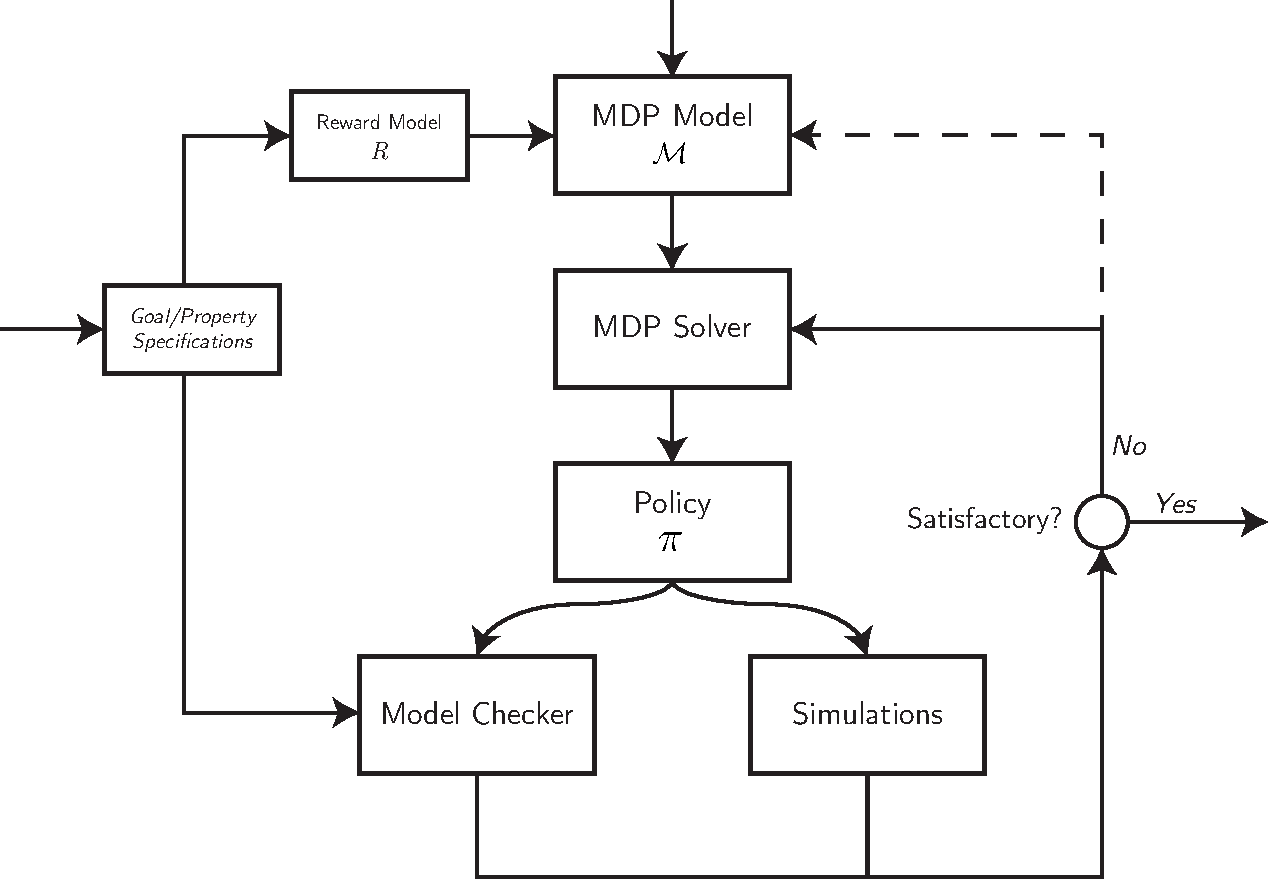
\includegraphics[width=\textwidth]{mdp-planning-diagram}
	\caption{Block diagram of the generic routine employed in model-based MDP planning techniques.}
	\label{fig:model-based-routine}
\end{figure}
% Planning algorithms for MDPs
% Planning algorithms for POMDPs

% \subsection{Integrated Architectures}
% Dyna Architecture -- combines model-learning and direct/value-based approaches, applies these iteratively even in execution of the agent --> 'hybrid' approach?
	% See "Integrated Learning and Planning" Lecture sheets by David Silver	[Integrated Architecture]
	% 

% 7.9.2








% perceptual aliasing!!!!!!